\section{System Architecture}

The AI-Based Trip Planner Web Application is designed using a modular, layered architecture that separates user interaction, business logic, machine learning inference, and data persistence into distinct components. This separation ensures maintainability, scalability, and testability of each system layer.

\begin{figure}[H]
    \centering
    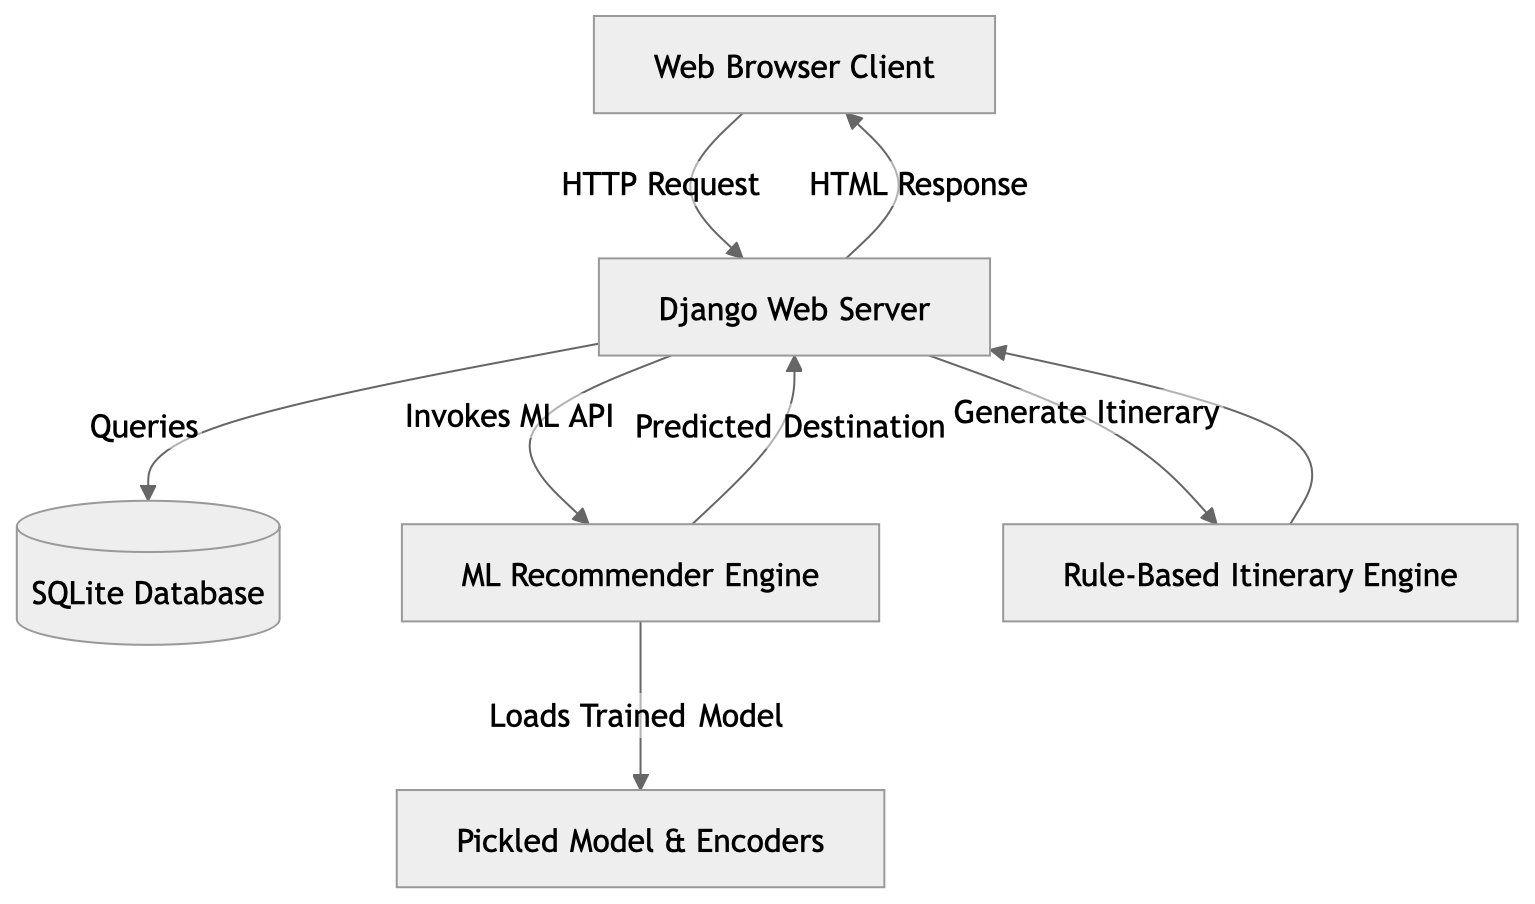
\includegraphics[width=0.9\textwidth,height=0.7\textheight,keepaspectratio]{images/High-Level System Architecture.png}
    \caption{High-Level System Architecture}
    \label{fig:system-architecture}
\end{figure}

The architecture consists of the following layers:

\begin{itemize}
    \item \textbf{Presentation Layer}: HTML5, CSS3, and JavaScript templates rendered through Django's template engine, providing responsive and interactive user interfaces.
    \item \textbf{Application Layer}: Django views and URL routing handle HTTP request processing, authentication, session management, and template rendering.
    \item \textbf{API Layer}: Django REST Framework exposes RESTful endpoints for frontend-backend communication, enabling JSON-based request and response handling.
    \item \textbf{Machine Learning Layer}: Pre-trained Decision Tree model loaded via Joblib for real-time destination prediction and itinerary generation.
    \item \textbf{Data Layer}: SQLite3 database accessed through Django's ORM for storing user accounts, trip records, and related data.
\end{itemize}

\section{User Interaction Flow}

The system follows a structured user interaction sequence from input submission to itinerary delivery:

\begin{figure}[H]
    \centering
    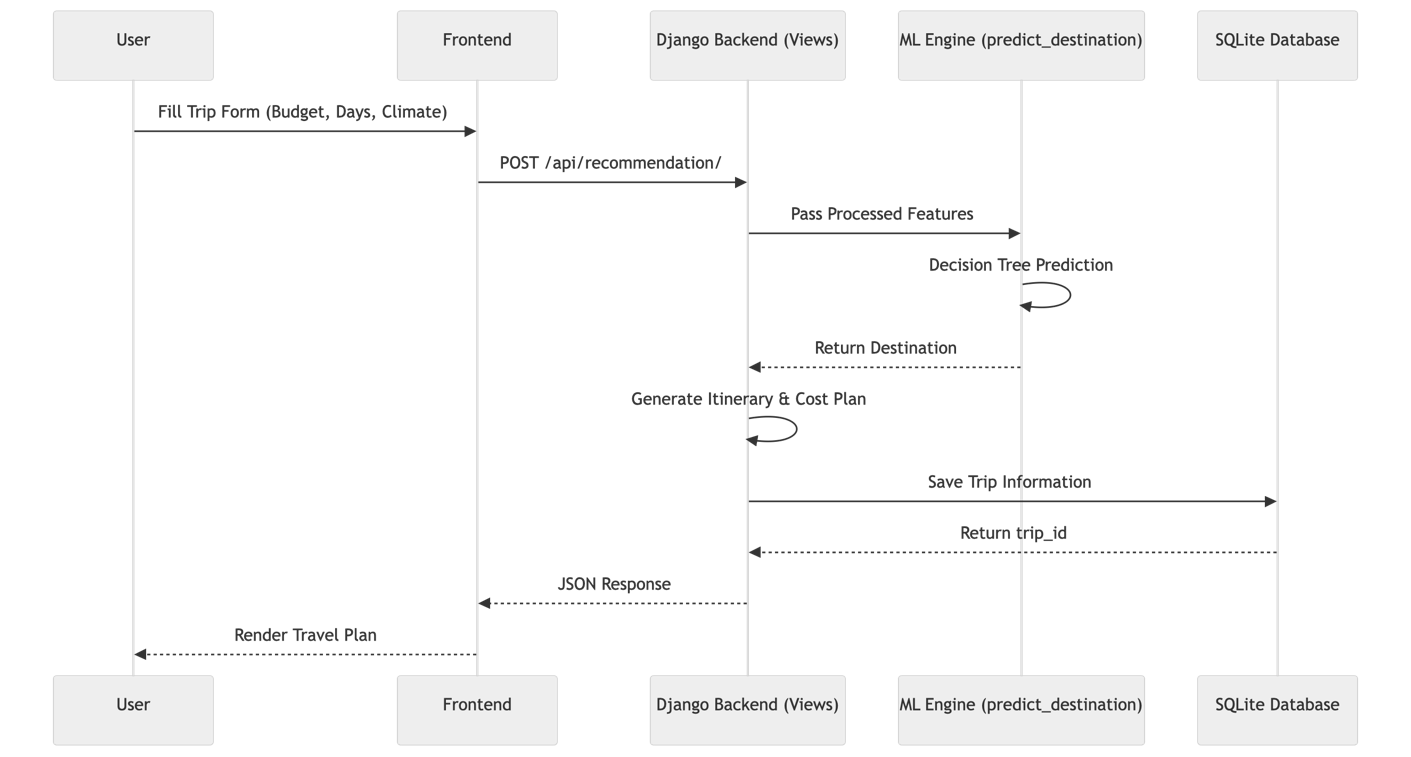
\includegraphics[width=0.9\textwidth,height=0.7\textheight,keepaspectratio]{images/User Interaction Sequence Diagram.png}
    \caption{User Interaction Sequence Diagram}
    \label{fig:user-interaction}
\end{figure}

\section{Database Design}

\subsection{Entity Relationship Diagram}

The database design consists of two primary entities: \texttt{USER} and \texttt{TRIP}. The relationship is one-to-many, where one user can have multiple associated trip records.

\begin{figure}[H]
    \centering
    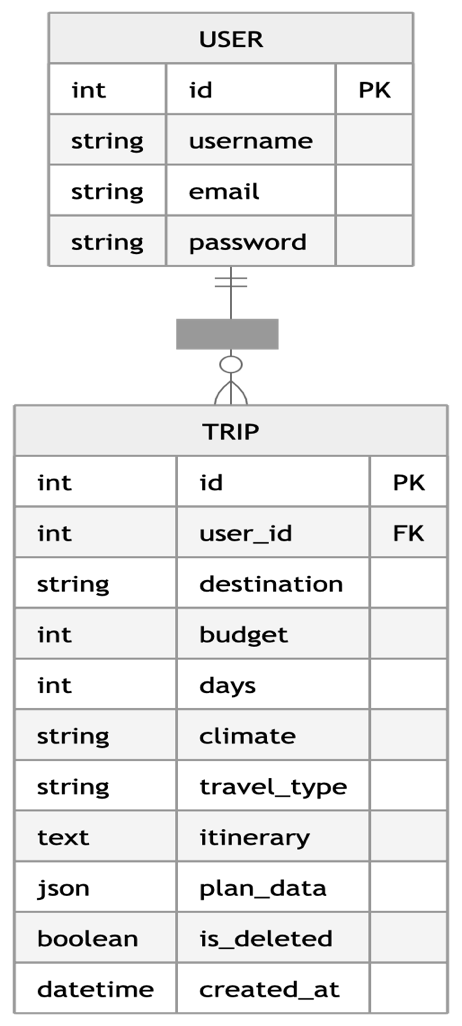
\includegraphics[width=0.9\textwidth,height=0.65\textheight,keepaspectratio]{images/Entity Relationship Diagram (ERD).png}
    \caption{Entity Relationship Diagram (ERD)}
    \label{fig:erd}
\end{figure}

\subsection{USER Entity}

The \texttt{USER} table stores authentication and account-related information. Attributes include:

\begin{itemize}
    \item \textbf{id}: Unique primary key
    \item \textbf{username}: User login identifier
    \item \textbf{email}: Registered email address
    \item \textbf{password}: Encrypted user password (managed by Django's \texttt{AbstractUser})
\end{itemize}

\subsection{TRIP Entity}

The \texttt{TRIP} table stores all generated travel plans and itinerary information. Attributes include:

\begin{itemize}
    \item \textbf{destination}: Predicted destination name
    \item \textbf{budget}: User-specified travel budget (INR)
    \item \textbf{days}: Trip duration in days
    \item \textbf{climate}: Preferred climate type (Hot, Cold, Moderate)
    \item \textbf{travel\_type}: Selected travel category (Adventure, Cultural, Family, Relaxation)
    \item \textbf{itinerary}: Generated day-wise schedule (text)
    \item \textbf{plan\_data}: JSON-formatted structured trip data including cost breakdown
    \item \textbf{is\_deleted}: Soft-delete status flag
    \item \textbf{deleted\_at}: Timestamp for soft-deletion event
    \item \textbf{created\_at}: Timestamp of trip creation
\end{itemize}

\section{Technology Stack}

The AI-Based Trip Planner Web Application utilizes a combination of backend frameworks, machine learning libraries, frontend technologies, and database systems to provide a scalable and intelligent travel planning platform.

\begin{table}[H]
    \centering
    \caption{Technology Stack Breakdown}
    \label{tab:tech-stack}
    \begin{tabularx}{\textwidth}{@{} l l X @{}}
        \toprule
        \textbf{Component} & \textbf{Technology} & \textbf{Purpose} \\
        \midrule
        Backend            & Python, Django           & Web framework, request routing, and ORM handling \\
        Machine Learning   & Scikit-Learn, Pandas     & Data preprocessing and ML prediction model \\
        Database           & SQLite3                  & Persistent relational data storage \\
        Frontend           & HTML5, CSS3, JavaScript  & User interface rendering and interaction \\
        API Framework      & Django REST Framework    & JSON REST APIs and request serialization \\
        Model Serialization & Joblib                  & Saving and reloading trained ML model files \\
        Version Control    & Git                      & Source code versioning and management \\
        \bottomrule
    \end{tabularx}
\end{table}

\subsection{Backend Technologies}

The backend is implemented using \textbf{Python} and \textbf{Django} \cite{django2026}. Django provides secure authentication, database abstraction through ORM, URL routing, middleware support, and template rendering functionalities. Key advantages include:

\begin{itemize}
    \item Rapid development through built-in utilities
    \item Built-in security (CSRF protection, password hashing)
    \item Scalable and modular architecture
    \item Easy database integration through ORM
\end{itemize}

\subsection{Machine Learning Technologies}

The machine learning module uses \textbf{Scikit-learn} \cite{pedregosa2011}, \textbf{Pandas} \cite{mckinney2010}, and \textbf{NumPy} for:

\begin{itemize}
    \item Data preprocessing and cleaning
    \item Categorical label encoding
    \item Decision Tree classifier training
    \item Real-time prediction inference
\end{itemize}
